\subsection{バッテリ}
バッテリは公称電圧7.6V,放電容量3900mAhのClyde Space社の30Whr Standalone CubeSat Batteryを購入した(図\ref{fig3_1_bat}).バッテリの電気・構造的特性を表\ref{table3_1_bat_spec}に,絶対最大定格を表\ref{table3_1_bat_max}に示す.このバッテリパックは2直3並列(2S3P)のリチウムポリマー電池であり,UN勧告適合品,NASA標準EP-Wi-032適合品である.

\begin{figure}[htbp]
	\begin{center}
		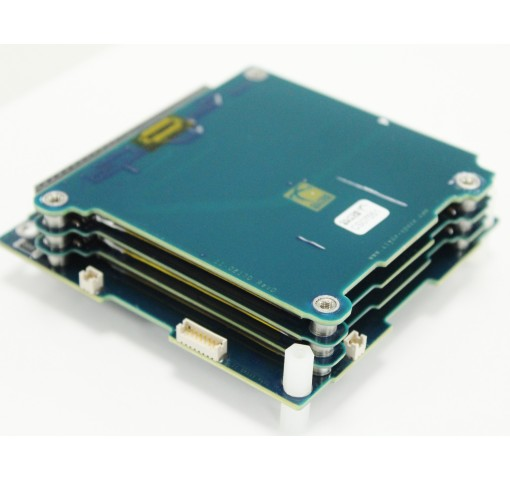
\includegraphics[width=0.5\linewidth]{./03/fig/battery.jpg}
		\caption{30Whr Standalone CubeSat Battery (c)Clyde Space}
		\label{fig3_1_bat}
	\end{center}
\end{figure}

\begin{table}[htbp]
	\begin{center}
		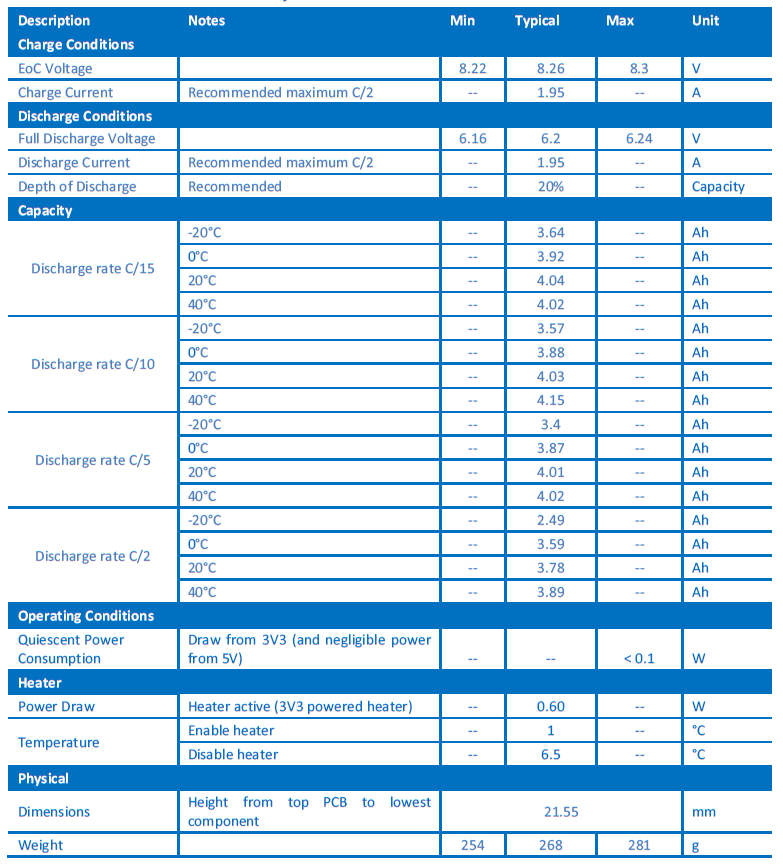
\includegraphics[width=0.9\linewidth]{./03/fig/battery_spec.png}
		\caption{30Whr}
		\label{table3_1_bat_spec}
	\end{center}
\end{table}


\begin{table}
	\caption{Maximum Ratings of the Battery}
	\label{table3_1_bat_max}
	\centering
	\begin{tabular}{ccccc}
		\hline \hline
		\multicolumn{5}{c}{Max Ratings Over Operating Temperature Range (Unless Otherwise Stated)}\\
		&&BCR  & Value  &  Unit  \\
		\hline
		\multirow{3}{*}{Charge Limits}&Voltage&max&8.4&V\\
		&Current&max&6&A\\
		&Current Rate& max &1.53C &Fraction of Capacity\\
		\hline
		\multirow{3}{*}{Discharge Limits}&Voltage&max&6.2&V\\
		&Current&max&6&A\\
		&Current Rate& max &1.53C &Fraction of Capacity\\
		\hline
		\multicolumn{2}{c}{Operating Temperature}&\multicolumn{2}{c}{ -10 to 50} & °C\\
		\multicolumn{2}{c}{\multirow{3}{*}{Storage Temperature}}&\multicolumn{2}{c}{1 Year: -20 to +20}&\multirow{3}{*}{°C}\\
		&&\multicolumn{2}{c}{3 Months: -20 to +45}&\\
		&&\multicolumn{2}{c}{1 Month: -20 to +60}&\\
		\multicolumn{2}{c}{Vacuum}&\multicolumn{2}{c}{10-5}&torr\\
		\multicolumn{2}{c}{Vibration}&\multicolumn{2}{c}{To [RD-3]}\\
		\hline
	\end{tabular}
\end{table}
	




本バッテリにはセルレベルの過電流,過充電,過放電保護回路,および1並列ごとの過電流保護回路が組み込まれている.これらの保護機能については,メーカーから試験報告書を入手し,さらに本衛星開発チームで環境試験(振動,衝撃)前後での充放電特性を測定した.

付録かな

ヒータが組み込まれており0℃以下で作用する.この機能は無効にすることもできた.さらに温度関係なく制御可能な自作ヒータを貼り付けた.

FMおよびEMにおいてはバッテリの$\mathrm{I^{2}C}$ラインの故障が生じたために,組み込まれていた機能としてのテレメトリ取得が不可能となった.バッテリの電圧,温度取得等の情報は別ラインで取得可能にしていた.


\begin{figure}[htbp]
	\begin{center}
		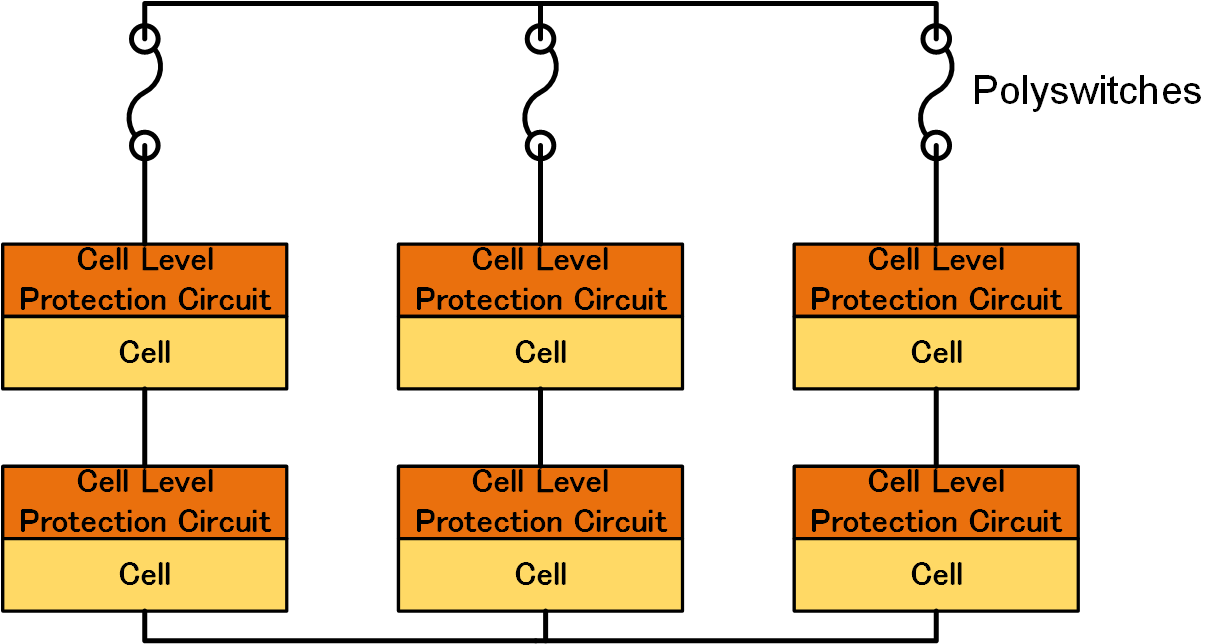
\includegraphics[width=0.5\linewidth]{./03/fig/BAT.png}
		\caption{Integrated EPS and Battery Protection Architecture 転載}
		\label{mir}
	\end{center}
\end{figure}

\begin{figure}[htbp]
	\begin{center}
		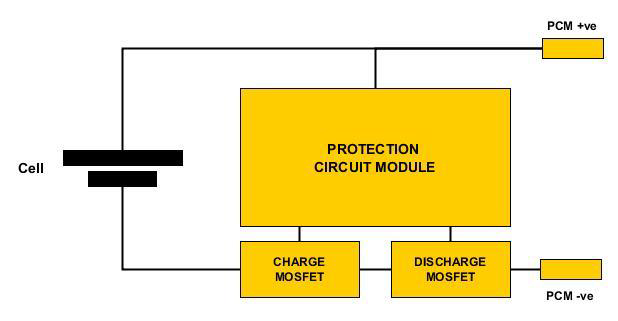
\includegraphics[width=0.5\linewidth]{./03/fig/cell_protection.png}
		\caption{Cell level protection circuit schematic 転載}
		\label{cell_p}
	\end{center}
\end{figure}

\begin{figure}[htbp]
	\begin{center}
		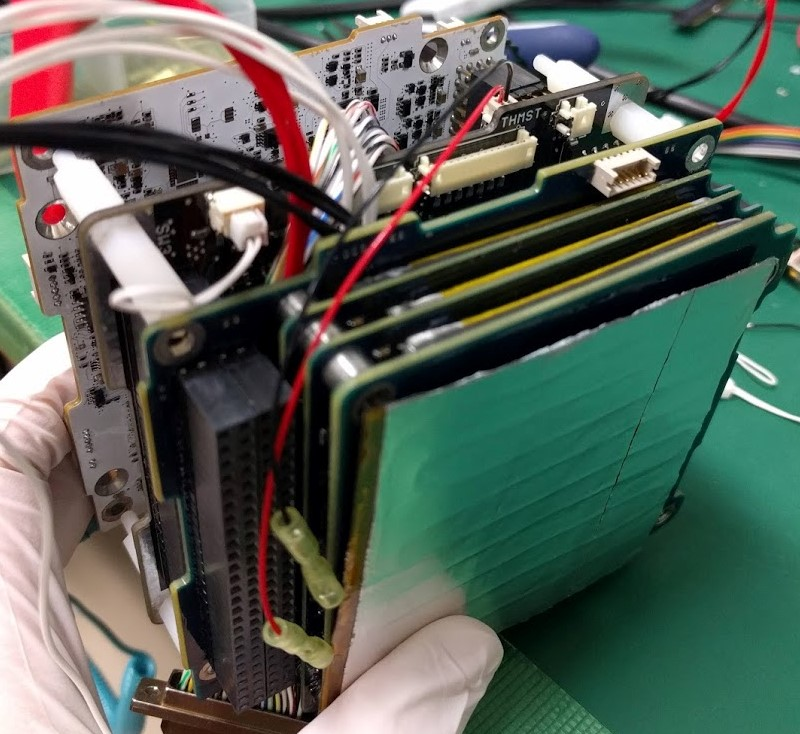
\includegraphics[width=0.5\linewidth]{./03/fig/heater.jpg}
		\caption{Cell level protection circuit schematic 転載}
		\label{cell_p}
	\end{center}
\end{figure}
